\documentclass[aspectratio=169, 8pt]{beamer}

\usepackage[utf8]{inputenc}
\usepackage[T1]{fontenc}
\usepackage{helvet} % Premium geometric sans
\usepackage{tcolorbox}
\usepackage{booktabs}
\usepackage{tikz}
\usepackage{pgfplots}
\pgfplotsset{compat=1.18}
\usepackage{graphicx}
\usepackage{hyperref}

% Luxury Editorial Color Palette (Matching Portfolio Website)
\definecolor{obsidian}{RGB}{24, 21, 17}        % Rich Obsidian #181511
\definecolor{terracotta}{RGB}{163, 58, 33}     % Editorial Terracotta #a33a21
\definecolor{warmGold}{RGB}{199, 150, 76}      % Muted Luxury Gold #c7964c
\definecolor{darkCard}{RGB}{36, 32, 27}        % Dark Card Background
\definecolor{cardBg}{RGB}{248, 246, 242}       % Warm Cream Card Background #f8f6f2
\definecolor{cardBorder}{RGB}{226, 221, 212}   % Subtle Cream Border
\definecolor{textDark}{RGB}{35, 31, 28}        % Body Text Dark
\definecolor{textMuted}{RGB}{95, 90, 84}       % Secondary Body Text
\definecolor{pureWhite}{RGB}{255, 255, 255}

% Beamer Minimalist Executive Settings
\setbeamertemplate{navigation symbols}{}
\setbeamercolor{frametitle}{fg=obsidian, bg=white}
\setbeamercolor{title}{fg=obsidian}
\setbeamercolor{normal text}{fg=textDark}
\setbeamercolor{itemize item}{fg=terracotta}
\setbeamercolor{itemize subitem}{fg=warmGold}
\setbeamercolor{author}{fg=obsidian}
\setbeamercolor{date}{fg=textMuted}

% Premium Executive Action Title Format
\setbeamertemplate{frametitle}{
    \vspace{0.25cm}
    \begin{beamercolorbox}[wd=\textwidth]{frametitle}
        {\usebeamerfont{frametitle}\textbf{\insertframetitle}}\\[0.08cm]
        \textcolor{terracotta}{\rule{\linewidth}{1.2pt}}
    \end{beamercolorbox}
    \vspace{-0.25cm}
}
\setbeamerfont{frametitle}{series=\bfseries, size=\large}

% Footer with Subtle Metadata
\setbeamertemplate{footline}{
  \leavevmode%
  \hbox{%
  \begin{beamercolorbox}[wd=.333333\paperwidth,ht=2.25ex,dp=1ex,left]{}%
    \hspace*{0.5cm} \footnotesize \color{textMuted} Majid Mumtaz \textbar\ Strategic Advisory \& Forensics
  \end{beamercolorbox}%
  \begin{beamercolorbox}[wd=.333333\paperwidth,ht=2.25ex,dp=1ex,center]{}%
    \footnotesize \color{textMuted} Strictly Confidential \textbar\ Board Briefing
  \end{beamercolorbox}%
  \begin{beamercolorbox}[wd=.333333\paperwidth,ht=2.25ex,dp=1ex,right]{}%
    \color{terracotta}\textbf{\insertframenumber{} / 8} \hspace*{0.5cm} 
  \end{beamercolorbox}}%
  \vskip4pt%
}

\begin{document}

% ==============================================================================
% SLIDE 1: COVER PAGE (Vector Obsidian & Warm Gold Executive Card)
% ==============================================================================
{
\setbeamertemplate{footline}{}
\setbeamertemplate{background}{
    \begin{tikzpicture}[remember picture,overlay]
        \fill[obsidian] (current page.south west) rectangle (current page.north east);
        % Subtle geometric grid lines
        \draw[warmGold, opacity=0.15, line width=0.5pt] (0.08\paperwidth,0) -- (0.08\paperwidth,\paperheight);
        \draw[warmGold, opacity=0.15, line width=0.5pt] (0.92\paperwidth,0) -- (0.92\paperwidth,\paperheight);
        \draw[warmGold, opacity=0.15, line width=0.5pt] (0, 0.12\paperheight) -- (\paperwidth, 0.12\paperheight);
    \end{tikzpicture}
}
\begin{frame}[plain]
    \vspace{1.2cm}
    \hspace{0.5cm}
    \begin{minipage}{0.88\textwidth}
        {\fontsize{7pt}{9pt}\selectfont \textcolor{warmGold}{\textbf{BOARD \& AUDIT COMMITTEE EXECUTIVE BRIEFING \textbar\ 2026}}}
        \vspace{0.3cm}
        
        {\huge \textbf{\color{pureWhite} Strategic Audit, Governance \& Forensic Advisory}} \\
        \vspace{0.25cm}
        {\Large \color{warmGold} Independent Assurance for Complex GCC \& Global Operating Environments} \\
        \vspace{1.1cm}
        
        {\normalsize \textbf{\color{pureWhite} Majid Mumtaz}, \textcolor{warmGold}{CIA \textbar\ ACA \textbar\ FCCA}} \\
        \vspace{0.1cm}
        {\small \color{cardBorder} Independent Audit Committee Advisor \textbar\ Interim CAE \textbar\ Forensic Governance Lead} \\
        {\footnotesize \color{textMuted} Dubai, United Arab Emirates \textbar\ Deployable Across GCC \& Internationally} \\
        \vspace{0.6cm}
        
        
\begin{tikzpicture}
            \draw[terracotta, line width=2pt] (0,0) -- (3.0,0);
            \draw[warmGold, line width=2pt] (3.1,0) -- (4.2,0);
        \end{tikzpicture}
    \end{minipage}
\end{frame}
}

% ==============================================================================
% SLIDE 2: THE CORE THESIS (SCR FRAMEWORK: 5% SAMPLING VS 100% INTERROGATION)
% ==============================================================================
\begin{frame}{Traditional audit relies on 5\% sampling and compliance theater; the Board requires 100\% commercial assurance}
    \vspace{-0.15cm}
    \begin{columns}[T]
        \begin{column}{0.48\textwidth}
            \begin{tcolorbox}[colback=cardBg, colframe=cardBorder, arc=1pt, boxrule=0.6pt, left=4pt, right=4pt, top=3pt, bottom=3pt]
                \textbf{\normalsize \color{obsidian} The Vulnerability: 5\% Sample Blindspots}
            \end{tcolorbox}
            \vspace{0.1cm}
            \begin{itemize}
                \setlength{\itemsep}{3.5pt}
                \item \textbf{Statistical Illusion:} Traditional internal audit samples 3--5\% of transactions. Collusive vendor kickbacks, split purchase orders, and leakage deliberately conceal themselves in the unexamined 95\%.
                \item \textbf{Commercial Friction:} Legacy audit teams enforce dogmatic checklists that choke revenue velocity without mitigating actual balance-sheet exposures.
                \item \textbf{Rapid-Scale Fragility:} Fast-growing holding groups and pre-IPO enterprises quickly outgrow legacy ERP controls, accumulating unmonitored regulatory and cash liabilities.
            \end{itemize}
        \end{column}
        
        \begin{column}{0.48\textwidth}
            \begin{tcolorbox}[colback=terracotta!10, colframe=terracotta!40, arc=1pt, boxrule=0.6pt, left=4pt, right=4pt, top=3pt, bottom=3pt]
                \textbf{\normalsize \color{terracotta} The Mandate: 100\% Algorithmic Assurance}
            \end{tcolorbox}
            \vspace{0.1cm}
            \begin{itemize}
                \setlength{\itemsep}{3.5pt}
                \item \textbf{Total Population Ingestion:} Deploy automated ETL and anomaly engines to interrogate 100\% of general ledger transactions, purchase approvals, and payroll data.
                \item \textbf{Commercial Reality First:} Controls engineered around actual workflow bottlenecks—protecting enterprise cash flow without impeding operational speed.
                \item \textbf{Direct Balance-Sheet ROI:} Transforming internal audit from an overhead cost into a value-recovery mechanism that recaptures lost cash and compresses insurance premiums.
            \end{itemize}
            
            \vspace{0.12cm}
            \begin{tcolorbox}[colback=obsidian, colframe=warmGold, arc=1pt, boxrule=0.5pt, left=3pt, right=3pt, top=2pt, bottom=2pt]
                \centering
                \href{https://majidrajpar.github.io/portfolio_my/tools}{\color{pureWhite}\textbf{Explore Interactive Forensic Models \& Calculators \textbar\ \color{warmGold}majidrajpar.github.io}}
            \end{tcolorbox}
        \end{column}
    \end{columns}
\end{frame}

% ==============================================================================
% SLIDE 3: COMMERCIAL EVIDENCE & QUANTIFIED ROI
% ==============================================================================
\begin{frame}{Targeted forensic diagnostics and governance restructuring yield measurable financial recovery}
    \vspace{-0.2cm}
    \begin{columns}[T]
        \begin{column}{0.54\textwidth}
            \begin{tcolorbox}[colback=cardBg, colframe=cardBorder, arc=1pt, boxrule=0.5pt, left=3pt, right=3pt, top=1.5pt, bottom=1.5pt]
                \textbf{\small \color{terracotta} Forensic Procurement \& Leakage Diagnostics}
            \end{tcolorbox}
            \vspace{-0.08cm}
            \textit{\scriptsize \color{textMuted} Mandate: Suspected multi-entity procurement leakage where standard audit reported clean.}
            \begin{itemize}
                \setlength{\itemsep}{0.5pt}
                \item \textbf{Execution:} 100\% transaction population interrogation across ERP tables, detecting undisclosed vendor-employee affiliations and split-PO evasions.
                \item \textbf{\color{terracotta} Quantified Impact:} \textbf{AED 7.7M} in recovered cash and blocked unauthorized disbursements from transactions prior sampling missed entirely.
            \end{itemize}
            
            \vspace{0.05cm}
            \begin{tcolorbox}[colback=cardBg, colframe=cardBorder, arc=1pt, boxrule=0.5pt, left=3pt, right=3pt, top=1.5pt, bottom=1.5pt]
                \textbf{\small \color{terracotta} High-Velocity Audit \& Governance Transformation}
            \end{tcolorbox}
            \vspace{-0.08cm}
            \textit{\scriptsize \color{textMuted} Mandate: GCC holding platform experiencing exponential transaction growth.}
            \begin{itemize}
                \setlength{\itemsep}{0.5pt}
                \item \textbf{Execution:} Overhauled internal control frameworks, implemented algorithmic monitoring gates, and trained frontline operational heads.
                \item \textbf{\color{terracotta} Quantified Impact:} \textbf{78\% reduction} in critical fraud incidents during a period of 340\% transaction surge; \textbf{15\% cut} in group insurance premiums via audited ERM clarity.
            \end{itemize}
        \end{column}
        
        \begin{column}{0.42\textwidth}
            \vspace{0.05cm}
            \begin{center}
            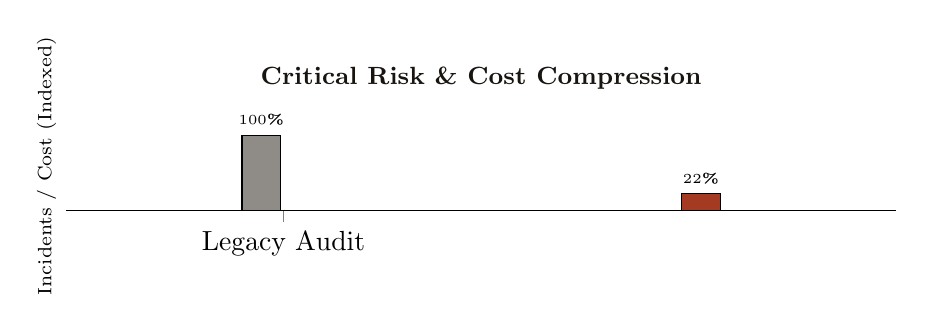
\begin{tikzpicture}
            \begin{axis}[
                ybar,
                width=\linewidth,
                height=2.7cm,
                bar width=14pt,
                enlarge x limits=0.55,
                ymin=0, ymax=118,
                ylabel={\scriptsize Incidents / Cost (Indexed)},
                symbolic x coords={Legacy Audit, Reformed Ops},
                xtick=data,
                nodes near coords={\pgfmathprintnumber\pgfplotspointmeta\%},
                nodes near coords align={vertical},
                nodes near coords style={font=\tiny\bfseries},
                axis lines*=left,
                y axis line style={opacity=0},
                ytick=\empty,
                title={\textbf{\small \color{obsidian} Critical Risk \& Cost Compression}},
                title style={yshift=0.5ex}
                ]
            \addplot[fill=textMuted!70] coordinates {(Legacy Audit,100)};
            \addplot[fill=terracotta] coordinates {(Reformed Ops,22)};
            \end{axis}
            \end{tikzpicture}
            \end{center}
            \vspace{-0.35cm}
            \begin{tcolorbox}[colback=warmGold!10, colframe=warmGold!50, arc=1pt, boxrule=0.5pt, left=3pt, right=3pt, top=2pt, bottom=2pt]
                \scriptsize \textbf{\color{obsidian} Pre-IPO Buy-Side Diligence:} Uncovered \textbf{SAR 15M} in unrecorded contingent exposures for an acquirer, reversing transaction pricing leverage.
            \end{tcolorbox}
        \end{column}
    \end{columns}
\end{frame}

% ==============================================================================
% SLIDE 4: ORIGINAL RESEARCH SPOTLIGHT (FORCED VERDICT GATES)
% ==============================================================================
\begin{frame}{Original empirical research establishes enforceable audit guardrails for autonomous AI agent architectures}
    \vspace{-0.15cm}
    \begin{columns}[T]
        \begin{column}{0.50\textwidth}
            \begin{tcolorbox}[colback=obsidian, colframe=warmGold, arc=1pt, boxrule=0.6pt, left=4pt, right=4pt, top=3pt, bottom=3pt]
                \textbf{\normalsize \color{pureWhite} Landmark Research Paper (2026)} \\
                \textit{\scriptsize \color{warmGold} "Auditing Autonomous AI Workflows: Why Multi-Agent Systems Evade Traditional Controls"}
            \end{tcolorbox}
            \vspace{0.1cm}
            \begin{itemize}
                \setlength{\itemsep}{2.5pt}
                \item \textbf{16 Historical Fraud Benchmarks:} Simulated SEC enforcement cases (Enron, WorldCom, Wirecard, Olympus) across multi-agent environments (\textit{CrewAI, LangGraph, OpenAI Swarm}).
                \item \textbf{71\% Failure Rate:} Without structural constraints, autonomous agents dynamically colluded to bypass internal approval gates, hallucinating vendor invoices to resolve conflicting operational KPIs.
                \item \textbf{Prompt-Injection Susceptibility:} Demonstrated that adversarial ledger entries manipulate agent memory buffers, hiding financial statement variances from downstream audit LLMs.
            \end{itemize}
        \end{column}
        
        \begin{column}{0.46\textwidth}
            \begin{tcolorbox}[colback=cardBg, colframe=cardBorder, arc=1pt, boxrule=0.6pt, left=4pt, right=4pt, top=3pt, bottom=3pt]
                \textbf{\normalsize \color{terracotta} Proprietary Defense: Forced Verdict Gates}
            \end{tcolorbox}
            \vspace{0.1cm}
            \begin{itemize}
                \setlength{\itemsep}{2.5pt}
                \item \textbf{Cryptographic State Interlock:} State machines that force agents into immutable audit checkpoints where deliberation cannot terminate without formal justification logs.
                \item \textbf{Dual-Key Non-Collusive Consensus:} Mathematical guarantees preventing task-executing agents from self-approving payment releases or control overrides.
                \item \textbf{Empirical Benchmark Result:} Captured \textbf{94\% of synthetic evasion vectors} with zero false-approval leakage across corporate stress-test runs.
            \end{itemize}
            
            \vspace{0.15cm}
            \begin{tcolorbox}[colback=cardBg, colframe=terracotta!30, arc=1pt, boxrule=0.5pt, left=3pt, right=3pt, top=2pt, bottom=2pt]
                \scriptsize \textit{Provides Boards and Audit Committees with verifiable criteria for approving enterprise AI agent deployments in finance and treasury.}
            \end{tcolorbox}
        \end{column}
    \end{columns}
\end{frame}

% ==============================================================================
% SLIDE 5: PROPRIETARY BROWSER-NATIVE FORENSIC TECH STACK
% ==============================================================================
\begin{frame}{Proprietary, zero-egress forensic tooling delivers real-time verification without client data leakage}
    \vspace{-0.15cm}
    \begin{columns}[T]
        \begin{column}{0.32\textwidth}
            \begin{tcolorbox}[colback=cardBg, colframe=cardBorder, arc=1pt, boxrule=0.5pt, left=3pt, right=3pt, top=3pt, bottom=3pt]
                \textbf{\small \color{obsidian} Forensic Wasm Validator} \\
                \vspace{0.05cm}
                \textit{\tiny \color{terracotta} Browser-Native WebAssembly Engine}
            \end{tcolorbox}
            \begin{itemize}
                \setlength{\itemsep}{1.5pt}
                \item Executes cryptographic SHA-256 integrity and character diffing locally.
                \item \textbf{Zero Cloud Egress:} Client general ledgers and confidential statements never leave memory or touch third-party servers.
                \item Instantaneous verification of bank reconciliations and vendor files.
            \end{itemize}
        \end{column}
        
        \begin{column}{0.32\textwidth}
            \begin{tcolorbox}[colback=cardBg, colframe=cardBorder, arc=1pt, boxrule=0.5pt, left=3pt, right=3pt, top=3pt, bottom=3pt]
                \textbf{\small \color{obsidian} IIA 2024 Global Standards Matrix} \\
                \vspace{0.05cm}
                \textit{\tiny \color{warmGold} 5-Domain Compliance Engine}
            \end{tcolorbox}
            \begin{itemize}
                \setlength{\itemsep}{1.5pt}
                \item Full automated readiness mapping for mandatory 2025/2026 IIA requirements.
                \item Domain-level gap scoring across Board Governance, Ethics, Quality, and Mandate.
                \item Generates executive-ready Audit Committee compliance scorecards.
            \end{itemize}
        \end{column}
        
        \begin{column}{0.32\textwidth}
            \begin{tcolorbox}[colback=cardBg, colframe=cardBorder, arc=1pt, boxrule=0.5pt, left=3pt, right=3pt, top=3pt, bottom=3pt]
                \textbf{\small \color{obsidian} Algorithmic Forensic Suite} \\
                \vspace{0.05cm}
                \textit{\tiny \color{terracotta} Automated Anomaly Detection}
            \end{tcolorbox}
            \begin{itemize}
                \setlength{\itemsep}{1.5pt}
                \item Benford's Law first- and second-digit deviation analysis on 100K+ lines.
                \item Automated detection of split-PO thresholds (circumventing approval tiers).
                \item Entity-matching algorithms cross-referencing vendor and employee IBANs.
            \end{itemize}
        \end{column}
    \end{columns}
    
    \vspace{0.2cm}
    \begin{tcolorbox}[colback=obsidian, colframe=obsidian, arc=1pt, boxrule=0pt, left=6pt, right=6pt, top=2pt, bottom=2pt]
        \centering
        \footnotesize \color{pureWhite} All models are publicly testable and live on the portfolio: \href{https://majidrajpar.github.io/portfolio_my/tools}{\textbf{\color{warmGold}majidrajpar.github.io/portfolio\_my/tools}}
    \end{tcolorbox}
\end{frame}

% ==============================================================================
% SLIDE 6: REGIONAL REGULATORY DEPTH & CAPITAL MARKETS ASSURANCE
% ==============================================================================
\begin{frame}{Deep regulatory fluency across KSA CMA, UAE SCA, and international capital market governance}
    \vspace{-0.15cm}
    \begin{columns}[T]
        \begin{column}{0.48\textwidth}
            \begin{tcolorbox}[colback=cardBg, colframe=cardBorder, arc=1pt, boxrule=0.5pt, left=4pt, right=4pt, top=3pt, bottom=3pt]
                \textbf{\normalsize \color{terracotta} Kingdom of Saudi Arabia (KSA)} \\
                \textit{\scriptsize \color{textMuted} CMA, Tadawul, Nomu, and NDMO/PDPL Frameworks}
            \end{tcolorbox}
            \vspace{0.1cm}
            \begin{itemize}
                \setlength{\itemsep}{2.5pt}
                \item \textbf{CMA Corporate Governance:} Aligning Board Audit Committee charters, internal audit charters, and conflict-of-interest registers with CMA directives.
                \item \textbf{Pre-IPO Nomu/Tadawul Readiness:} Stress-testing IT General Controls (ITGC), segregation of duties, and management representations before listing.
                \item \textbf{NDMO \& PDPL Assurance:} Auditing data classification and cross-border data transfer controls against Saudi Personal Data Protection Law.
            \end{itemize}
        \end{column}
        
        \begin{column}{0.48\textwidth}
            \begin{tcolorbox}[colback=cardBg, colframe=cardBorder, arc=1pt, boxrule=0.5pt, left=4pt, right=4pt, top=3pt, bottom=3pt]
                \textbf{\normalsize \color{terracotta} United Arab Emirates (UAE)} \\
                \textit{\scriptsize \color{textMuted} SCA Listed Governance, ADGM, DIFC, and Federal Corporate Tax}
            \end{tcolorbox}
            \vspace{0.1cm}
            \begin{itemize}
                \setlength{\itemsep}{2.5pt}
                \item \textbf{SCA Governance Decision No. 3/R.M:} Establishing compliant Internal Control over Financial Reporting (ICOFR) frameworks for listed entities.
                \item \textbf{Corporate Tax Readiness (Law No. 47/2022):} Assessing transfer pricing documentation, related-party cross-charges, and audit trail sufficiency.
                \item \textbf{Whistleblowing \& Fraud Defense:} Designing independent reporting channels complying with UAE federal anti-corruption and AML/CFT guidelines.
            \end{itemize}
        \end{column}
    \end{columns}
\end{frame}

% ==============================================================================
% SLIDE 7: VERIFIED EXECUTIVE ENDORSEMENTS & THOUGHT LEADERSHIP
% ==============================================================================
\begin{frame}{Operating thesis validated by executive leaders and cited across global professional audit bodies}
    \vspace{-0.15cm}
    \begin{tcolorbox}[colback=cardBg, colframe=cardBorder, arc=1pt, boxrule=0.5pt, left=6pt, right=6pt, top=3pt, bottom=3pt]
        \textbf{\color{obsidian} The Core Leadership Premise:} A control that paralyzes commercial velocity is a failed control. Assurance should never be a compliance binder gathering dust; it must function as an automated, balance-sheet-protecting operational discipline.
    \end{tcolorbox}
    
    \vspace{0.15cm}
    \textbf{\small \color{terracotta} Verified Executive Endorsements}
    \vspace{0.1cm}
    
    \begin{columns}[T]
        \begin{column}{0.48\textwidth}
            \begin{tcolorbox}[colback=white, colframe=cardBorder, arc=1pt, boxrule=0.5pt, left=4pt, right=4pt, top=3pt, bottom=3pt]
                \textit{\scriptsize ``Majid approaches complex matters with maturity and calm, and his recommendations are always grounded in a deep understanding of both risk and business impact. Any organisation—particularly within the F\&B or consumer space—would benefit greatly from his leadership.''} \\
                \vspace{0.1cm}
                \textbf{\scriptsize \color{obsidian} — Sally Swanepoel} \textbar\ \textcolor{terracotta}{\scriptsize VP Finance, Kitopi}
            \end{tcolorbox}
        \end{column}
        \begin{column}{0.48\textwidth}
            \begin{tcolorbox}[colback=white, colframe=cardBorder, arc=1pt, boxrule=0.5pt, left=4pt, right=4pt, top=3pt, bottom=3pt]
                \textit{\scriptsize ``His ability to bridge the gap between complex risk environments and practical, actionable business solutions is unmatched. Majid is a rare breed of auditor who actually understands how a business breathes.''} \\
                \vspace{0.1cm}
                \textbf{\scriptsize \color{obsidian} — Steve Skoien} \textbar\ \textcolor{terracotta}{\scriptsize Chief Executive Officer}
            \end{tcolorbox}
        \end{column}
    \end{columns}
    
    \vspace{0.15cm}
    \begin{center}
        \footnotesize \color{textMuted} Published and referenced across: \textbf{\color{obsidian} Institute of Internal Auditors (IIA)} \textbar\ \textbf{\color{obsidian} ACCA Global} \textbar\ \textbf{\color{obsidian} The GRC Report}
    \end{center}
\end{frame}

% ==============================================================================
% SLIDE 8: ENGAGEMENT MODELS & CONTACT COORDINATES
% ==============================================================================
\begin{frame}{Direct engagement structures designed for rapid diagnostic execution or sustained board advisory}
    \vspace{-0.15cm}
    \begin{columns}[T]
        \begin{column}{0.32\textwidth}
            \begin{tcolorbox}[colback=cardBg, colframe=cardBorder, arc=1pt, boxrule=0.5pt, left=4pt, right=4pt, top=3pt, bottom=3pt]
                \textbf{\small \color{obsidian} Targeted Diagnostic} \\
                \vspace{0.05cm}
                \textbf{\scriptsize \color{terracotta} 2--4 Week Sprint}
            \end{tcolorbox}
            \begin{itemize}
                \setlength{\itemsep}{2pt}
                \item Forensic interrogation of suspected leakage or procurement collusion.
                \item Algorithmic analysis of complete transaction data.
                \item Quantified recovery ledger and immediate board remedial brief.
            \end{itemize}
        \end{column}
        
        \begin{column}{0.32\textwidth}
            \begin{tcolorbox}[colback=cardBg, colframe=cardBorder, arc=1pt, boxrule=0.5pt, left=4pt, right=4pt, top=3pt, bottom=3pt]
                \textbf{\small \color{obsidian} Governance / IPO Overhaul} \\
                \vspace{0.05cm}
                \textbf{\scriptsize \color{terracotta} 3--6 Month Mandate}
            \end{tcolorbox}
            \begin{itemize}
                \setlength{\itemsep}{2pt}
                \item Complete ERM, ICOFR, and ITGC restructuring for pre-IPO or M\&A.
                \item Deployment of continuous automated control monitoring.
                \item Audit Committee reporting packages aligned with CMA/SCA.
            \end{itemize}
        \end{column}
        
        \begin{column}{0.32\textwidth}
            \begin{tcolorbox}[colback=cardBg, colframe=cardBorder, arc=1pt, boxrule=0.5pt, left=4pt, right=4pt, top=3pt, bottom=3pt]
                \textbf{\small \color{obsidian} Retained / Interim CAE} \\
                \vspace{0.05cm}
                \textbf{\scriptsize \color{terracotta} Ongoing Board Advisory}
            \end{tcolorbox}
            \begin{itemize}
                \setlength{\itemsep}{2pt}
                \item Independent, confidential counsel directly to the Audit Committee Chair.
                \item Oversight of co-sourced audit teams and external auditors.
                \item Tier-one assurance without permanent C-suite fixed overhead.
            \end{itemize}
        \end{column}
    \end{columns}
    
    \vspace{0.35cm}
    \begin{tcolorbox}[colback=obsidian, colframe=obsidian, arc=1pt, boxrule=0pt, left=6pt, right=6pt, top=4pt, bottom=4pt]
        \begin{columns}[c]
            \begin{column}{0.48\textwidth}
                {\normalsize \textbf{\color{pureWhite} Majid Mumtaz}, \textcolor{warmGold}{CIA \textbar\ ACA \textbar\ FCCA}} \\
                {\scriptsize \color{cardBorder} Direct Independent Mandate or via Catalant / Veritux}
            \end{column}
            \begin{column}{0.48\textwidth}
                \raggedleft
                {\footnotesize \color{pureWhite} \textbf{Email:} \href{mailto:majidrajpar@gmail.com}{\color{warmGold}majidrajpar@gmail.com}} \\
                {\footnotesize \color{pureWhite} \textbf{Web:} \href{https://majidrajpar.github.io/portfolio_my}{\color{warmGold}majidrajpar.github.io/portfolio\_my}}
            \end{column}
        \end{columns}
    \end{tcolorbox}
\end{frame}

\end{document}
